\begin{frame}{Extras}
Extra Stuff...
\end{frame}


\begin{frame}{Congress/DAO Re-entrancy}
\begin{figure}
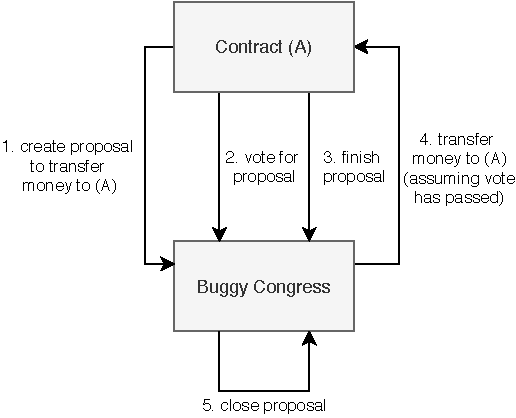
\includegraphics[scale=0.85]{media/congress-reentrancy.pdf}
\end{figure}
\end{frame}

\defverbatim[colored]\congresswellbehaved{
\begin{coq}
Definition cacts_preserved new_state resp_acts old_state msg :=
  num_cacts_in_state new_state + length resp_acts <=
  num_cacts_in_state old_state + proposal_cacts msg.

Lemma receive_state_well_behaved
      chain ctx state msg new_state resp_acts :
  receive chain ctx state msg = Some (new_state, resp_acts) ->
  cacts_preserved new_state resp_acts old_state msg.

QuickChick (
  {{fun _ _ => true}}
  Congress_Buggy.contract
  {{receive_state_well_behaved_P}}
).
\end{coq}
}
\begin{frame}{Congress/DAO Re-entrancy}{Safety Property}
\congresswellbehaved
\end{frame}

\begin{frame}{UniSwap Exploit}{Exchange Rate Formula}
\begin{enumerate}
    \item calculate the exact exchange rate
    \item send corresponding Ether to the caller
    \item transfer tokens to the liquidity contract
\end{enumerate}
The exchange rate formula:
\begin{equation*}
\begin{split}
getInputPrice &= \frac{Ts \cdot 997 \cdot ETHr}{Tr \cdot 1000 + Ts \cdot 997}\\
\text{where}&\\
Ts&: \text{nr. of tokens being sold by caller} \\
Tr&: \text{current token reserve held by the liquidity contract} \\
ETHr&: \text{current Ether reserve held by the liquidity contract}
\end{split}
\end{equation*}
\end{frame}

\begin{frame}{Dexter Exchange Protocol}
\begin{figure}
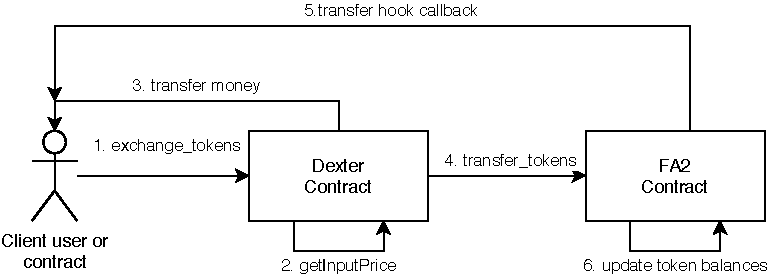
\includegraphics[scale=0.85]{media/Dexter-exchange-diagram.pdf}
\end{figure}
\end{frame}